\begin{figure}[htbp]
    \centering
    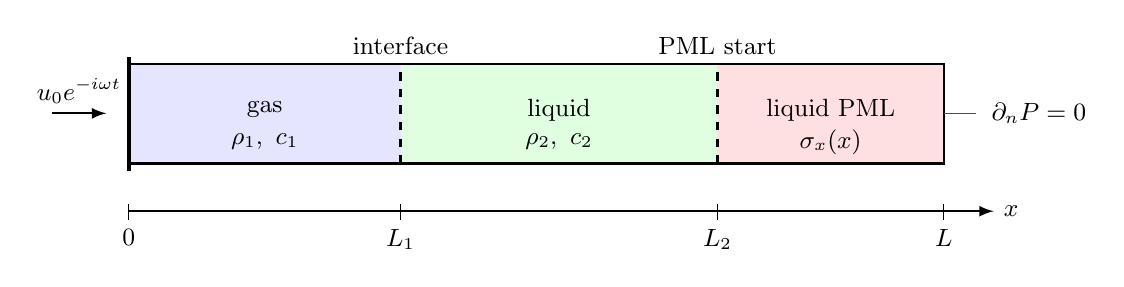
\begin{tikzpicture}[x=1.15cm,y=1.1cm,>=latex,font=\small]
        \def\xzero{0}
        \def\xone{3.0}
        \def\xtwo{6.5}
        \def\xthree{9.0}
        \def\h{1.15}

        \fill[blue!10] (\xzero,0) rectangle (\xone,\h);
        \fill[green!12] (\xone,0) rectangle (\xtwo,\h);
        \fill[red!12] (\xtwo,0) rectangle (\xthree,\h);
        \draw[thick] (\xzero,0) rectangle (\xthree,\h);
        \draw[thick,dashed] (\xone,0) -- (\xone,\h);
        \draw[thick,dashed] (\xtwo,0) -- (\xtwo,\h);

        \draw[very thick] (\xzero,-0.08) -- (\xzero,\h+0.08);
        \draw[->,thick] (-0.85,0.58) -- (-0.25,0.58)
            node[midway,above] {$u_0e^{-i\omega t}$};

        \node at (1.5,0.62) {gas};
        \node at (1.5,0.25) {$\rho_1,\ c_1$};
        \node at (4.75,0.62) {liquid};
        \node at (4.75,0.25) {$\rho_2,\ c_2$};
        \node at (7.75,0.62) {liquid PML};
        \node at (7.75,0.25) {$\sigma_x(x)$};

        \draw[->,thick] (\xzero,-0.55) -- (9.55,-0.55) node[right] {$x$};
        \foreach \x/\lab in
            {\xzero/$0$,\xone/$L_1$,\xtwo/$L_2$,\xthree/$L$}
        {
            \draw (\x,-0.47) -- (\x,-0.65);
            \node[below] at (\x,-0.65) {\lab};
        }
        \node[above] at (\xone,\h) {interface};
        \node[above] at (\xtwo,\h) {PML start};
        \draw[black!70] (\xthree,0.58) -- (9.35,0.58);
        \node[anchor=west] at (9.42,0.58) {$\partial_nP=0$};
    \end{tikzpicture}
    \caption{Configuration of the integrated one-dimensional layered-interface
    and directional-PML validation case.}
    \label{fig:combinedLayeredSchematic}
\end{figure}
